\documentclass{standalonex}
\usepackage{tikz}
\usetikzlibrary{arrows}

\begin{document}
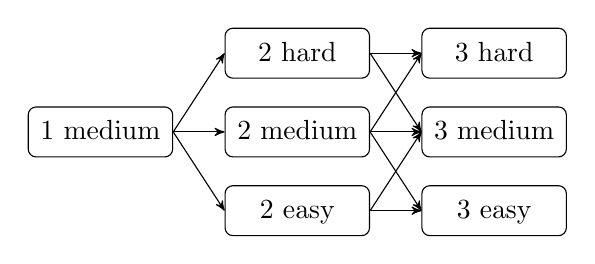
\begin{tikzpicture}[>=stealth',rounded corners=1mm,xscale=2.5,every node/.style={text width=1.6cm,text height=3mm,align=center,text depth=1mm}]
\node[draw,rectangle] (1) {1 medium};
\node[draw,rectangle] (2h) at (1,1) {2 hard};
\node[draw,rectangle] (2m) at (1,0) {2 medium};
\node[draw,rectangle] (2e) at (1,-1) {2 easy};
\node[draw,rectangle] (3h) at (2,1) {3 hard};
\node[draw,rectangle] (3m) at (2,0) {3 medium};
\node[draw,rectangle] (3e) at (2,-1) {3 easy};
\draw[->] (1.east) to (2h.west);
\draw[->] (1.east) to (2m.west);
\draw[->] (1.east) to (2e.west);
\draw[->] (2h.east) to (3h.west);
\draw[->] (2h.east) to (3m.west);
\draw[->] (2m.east) to (3h.west);
\draw[->] (2m.east) to (3m.west);
\draw[->] (2m.east) to (3e.west);
\draw[->] (2e.east) to (3m.west);
\draw[->] (2e.east) to (3e.west);
\end{tikzpicture}
\end{document}
